
%%%%%%%%%%%%%%%%%%%%%%%%%%%%%%%%%%%%%%%%%%%%%%%%%%%%%%%%%%%%%%%%%%%%%%%%%%%%%%%%
%% CAPITULO
%%%%%%%%%%%%%%%%%%%%%%%%%%%%%%%%%%%%%%%%%%%%%%%%%%%%%%%%%%%%%%%%%%%%%%%%%%%%%%%%
\chapterimage{chapter_head_2.pdf} % Chapter heading image

\chapter{Historia do samba de gafieira  (dança)}
\label{cap:sambagafieira}
\index{Dança!Samba de gafieira}


\section{Lundum (a dança do lundu)} 
\label{sec:lundu}
\index{Dança!Lundu}
O lundum é o estilo de dança que lhe corresponde ao gênero musical lundu \cite[pp. 18]{perna2002samba}.
Esta é uma dança, brasileira, de roda e umbigada; e teve sua origem no batuque dos bantos africanos,
e provavelmente foi trazida de Angola pelos escravos na segunda metade do século XVIII \cite[pp. 48]{tinhorao1986pequena} \cite[pp. 188]{dourado2004dicionario},
sendo que as primeiras referencias conhecidas se remontam a 1780 
descrevendo a dança como indecente e licenciosa \cite[pp. 51]{tinhorao1986pequena} \cite[pp. 19]{perna2002samba}.
Posteriormente foi introduzida aos salões das cortes do Brasil e Portugal, 
dançado elegantemente nas cortes, porem indecentemente pela gente comum   \cite[pp. 19]{perna2002samba} \cite[pp. 188]{dourado2004dicionario}.
No Brasil esta dança teve influencias da ``Modinha''(Portuguesa) e do ``Fandango''(Espanhol) \cite[pp. 188]{dourado2004dicionario}.

A partir de 1820 o lundum é apresentado, como dança de caráter libidinoso nos teatros de Baia, Pernambuco e Rio de Janeiro;
onde eram representados pequenos quadros cômicos, 
mostrando a umbigada e outras caraterísticas da dança \cite[pp. 19]{perna2002samba}.


\section{Maxixe (dança)}
\label{sec:maxixe}
\index{Dança!Maxixe}
Esta é uma dança urbana afro-brasileira \cite[pp. 4]{musicasambavariasdef1}, 
em compasso binário, surgida em Rio de Janeiro, 
na Cidade Nova e nos cabarés de Lapa \cite[pp. 465]{marcondes1977enciclopedia}  \cite[pp. 198]{dourado2004dicionario}, 
aproximadamente entre 1870 e 1880 \cite[pp. 58]{tinhorao1986pequena} \cite[pp. 465]{marcondes1977enciclopedia}  \cite[pp. 62]{reinato2010musica}.

A dança era considerada de baixe ralé pela sociedade local, 
pois era entendida como um modismo indecente das classes baixas, imoral como o Lundu \cite[pp. 198]{dourado2004dicionario}.
Esta dança recebeu influencias da polca \cite[pp. 198]{dourado2004dicionario} e 
da Habanera \cite[pp. 62]{reinato2010musica}.


O maxixe tinha uma boa quantidade de passos como: 
\begin{itemize} 
\item parafuso  \cite[pp. 68, 93, 129]{efege1974maxixe} \cite[pp. 465]{marcondes1977enciclopedia} \cite[pp. 62]{tinhorao1986pequena}, 
\item janela  \cite[pp. 129]{efege1974maxixe},
\item jocotó \cite[pp. 83, 96, 173]{efege1974maxixe},
\item saca-rolha \cite[pp. 465]{marcondes1977enciclopedia}, 
\item balão \cite[pp. 93]{efege1974maxixe} \cite[pp. 465]{marcondes1977enciclopedia}, 
\item balão apagado \cite[pp. 68]{efege1974maxixe} \cite[aproximadamente min. 11:35]{MaxixeDocumentario1},
\item balão caindo  \cite[pp. 129, 131]{efege1974maxixe} \cite[pp. 62]{tinhorao1986pequena},
\item corta-jaca  \cite[pp. 131]{efege1974maxixe},
\item urubu malandro  \cite[pp. 131]{efege1974maxixe},
\item sino \cite[pp. 68]{efege1974maxixe}, 
\item carrapeta  \cite[pp. 465]{marcondes1977enciclopedia}, 
\item corta-capim \cite[pp. 465]{marcondes1977enciclopedia} \cite[pp. 62]{tinhorao1986pequena}, 
\item cobrinha \cite[pp. 62]{tinhorao1986pequena},
\item maxixe puladinho \cite[pp. 177]{1920revista},
\item etc. 
\end{itemize}
Num principio o maxixe era dançado nas músicas de tango, havanera, polca e lundu; 
e só foi ate o final do século XIX que ganhou uma música com gênero próprio \cite[pp. 465]{marcondes1977enciclopedia},
criado pela fusão da polca, o schottisch e a mazurca \cite[pp. 58]{tinhorao1986pequena}.

No inícios do século XX o maxixe foi exportado e dançado na Europa, atingindo um grande sucesso, 
chegando a ser apresentado pelo dançarino ``Duque'' em Paris (1914) e em Londres (1922) \cite[pp. 465]{marcondes1977enciclopedia}.
Este dançarino é considerado o civilizador do maxixe \cite[pp. 129]{efege1974maxixe}.

Uma explicação muito interessante do maxixe é cantada pela atriz, Aurélia Delorme,
numa representação num quadro de revista, interpretando  ``Maxixe Aristocrático'' (1904, José Nunes), 
que arrancava aplausos e provocava pedidos de bis;
o seguinte texto indica sua pauta \cite[pp. 80-81]{efege1974maxixe} \cite{REIS2003}: 
\begin{citando}
O maxixe tem ciência,\\
ou pelo menos tem arte.\\
Para haver proficiência\\
basta mexer certa parte.\\
Pois o próprio Padre Santo,\\
sabendo o gosto que tem,\\
virá de Roma ao Brasil\\
dançar maxixe também.\\ 
\end{citando}



\section{Samba de gafieira (dança)}
\index{Dança!Samba de gafieira}
O samba de gafieira, como dança, descende principalmente do maxixe (dança),
que a sua vez foi gerado  pela união do  lundu, 
a polca e outras danças europeias.
Assim, misturando o maxixe com a ginga, e o ritmo de outras danças africanas, 
é que se obteve o samba dançado nas gafieiras \cite[pp. 139]{perna2002samba}, também chamado
samba de salão ou samba carioca \cite[pp. 50]{fornaciari1947aprender},
atualmente entenderíamos a este samba como o samba de gafieira (primigênio\footnote{
Primitivo; primordial; o primeiro da sua espécie. = PRIMÍGENO \cite{priberamprimigenio}.
}).




A Figura \ref{fig:formuladosambagafieira} mostra a árvore genealógico do samba de gafieira,
visto quando o samba (música) fez sua aparição nos salões de dança denominados no \AnoLivro~ como gafieiras.
\begin{figure}[h]
  \centering
  \begin{subfigure}[b]{0.52\textwidth}
    \centering
    \includegraphics[width=\textwidth]{chapters/cap-historia-sambagafieira/sambagafieiraformula.eps}
    \caption{Formação dos primeiros sambas dançados nas gafieiras ou samba de gafieira (primigênio).}
    \label{fig:formuladosambagafieira}
  \end{subfigure}
  ~~
  \begin{subfigure}[b]{0.37\textwidth}
    \centering
    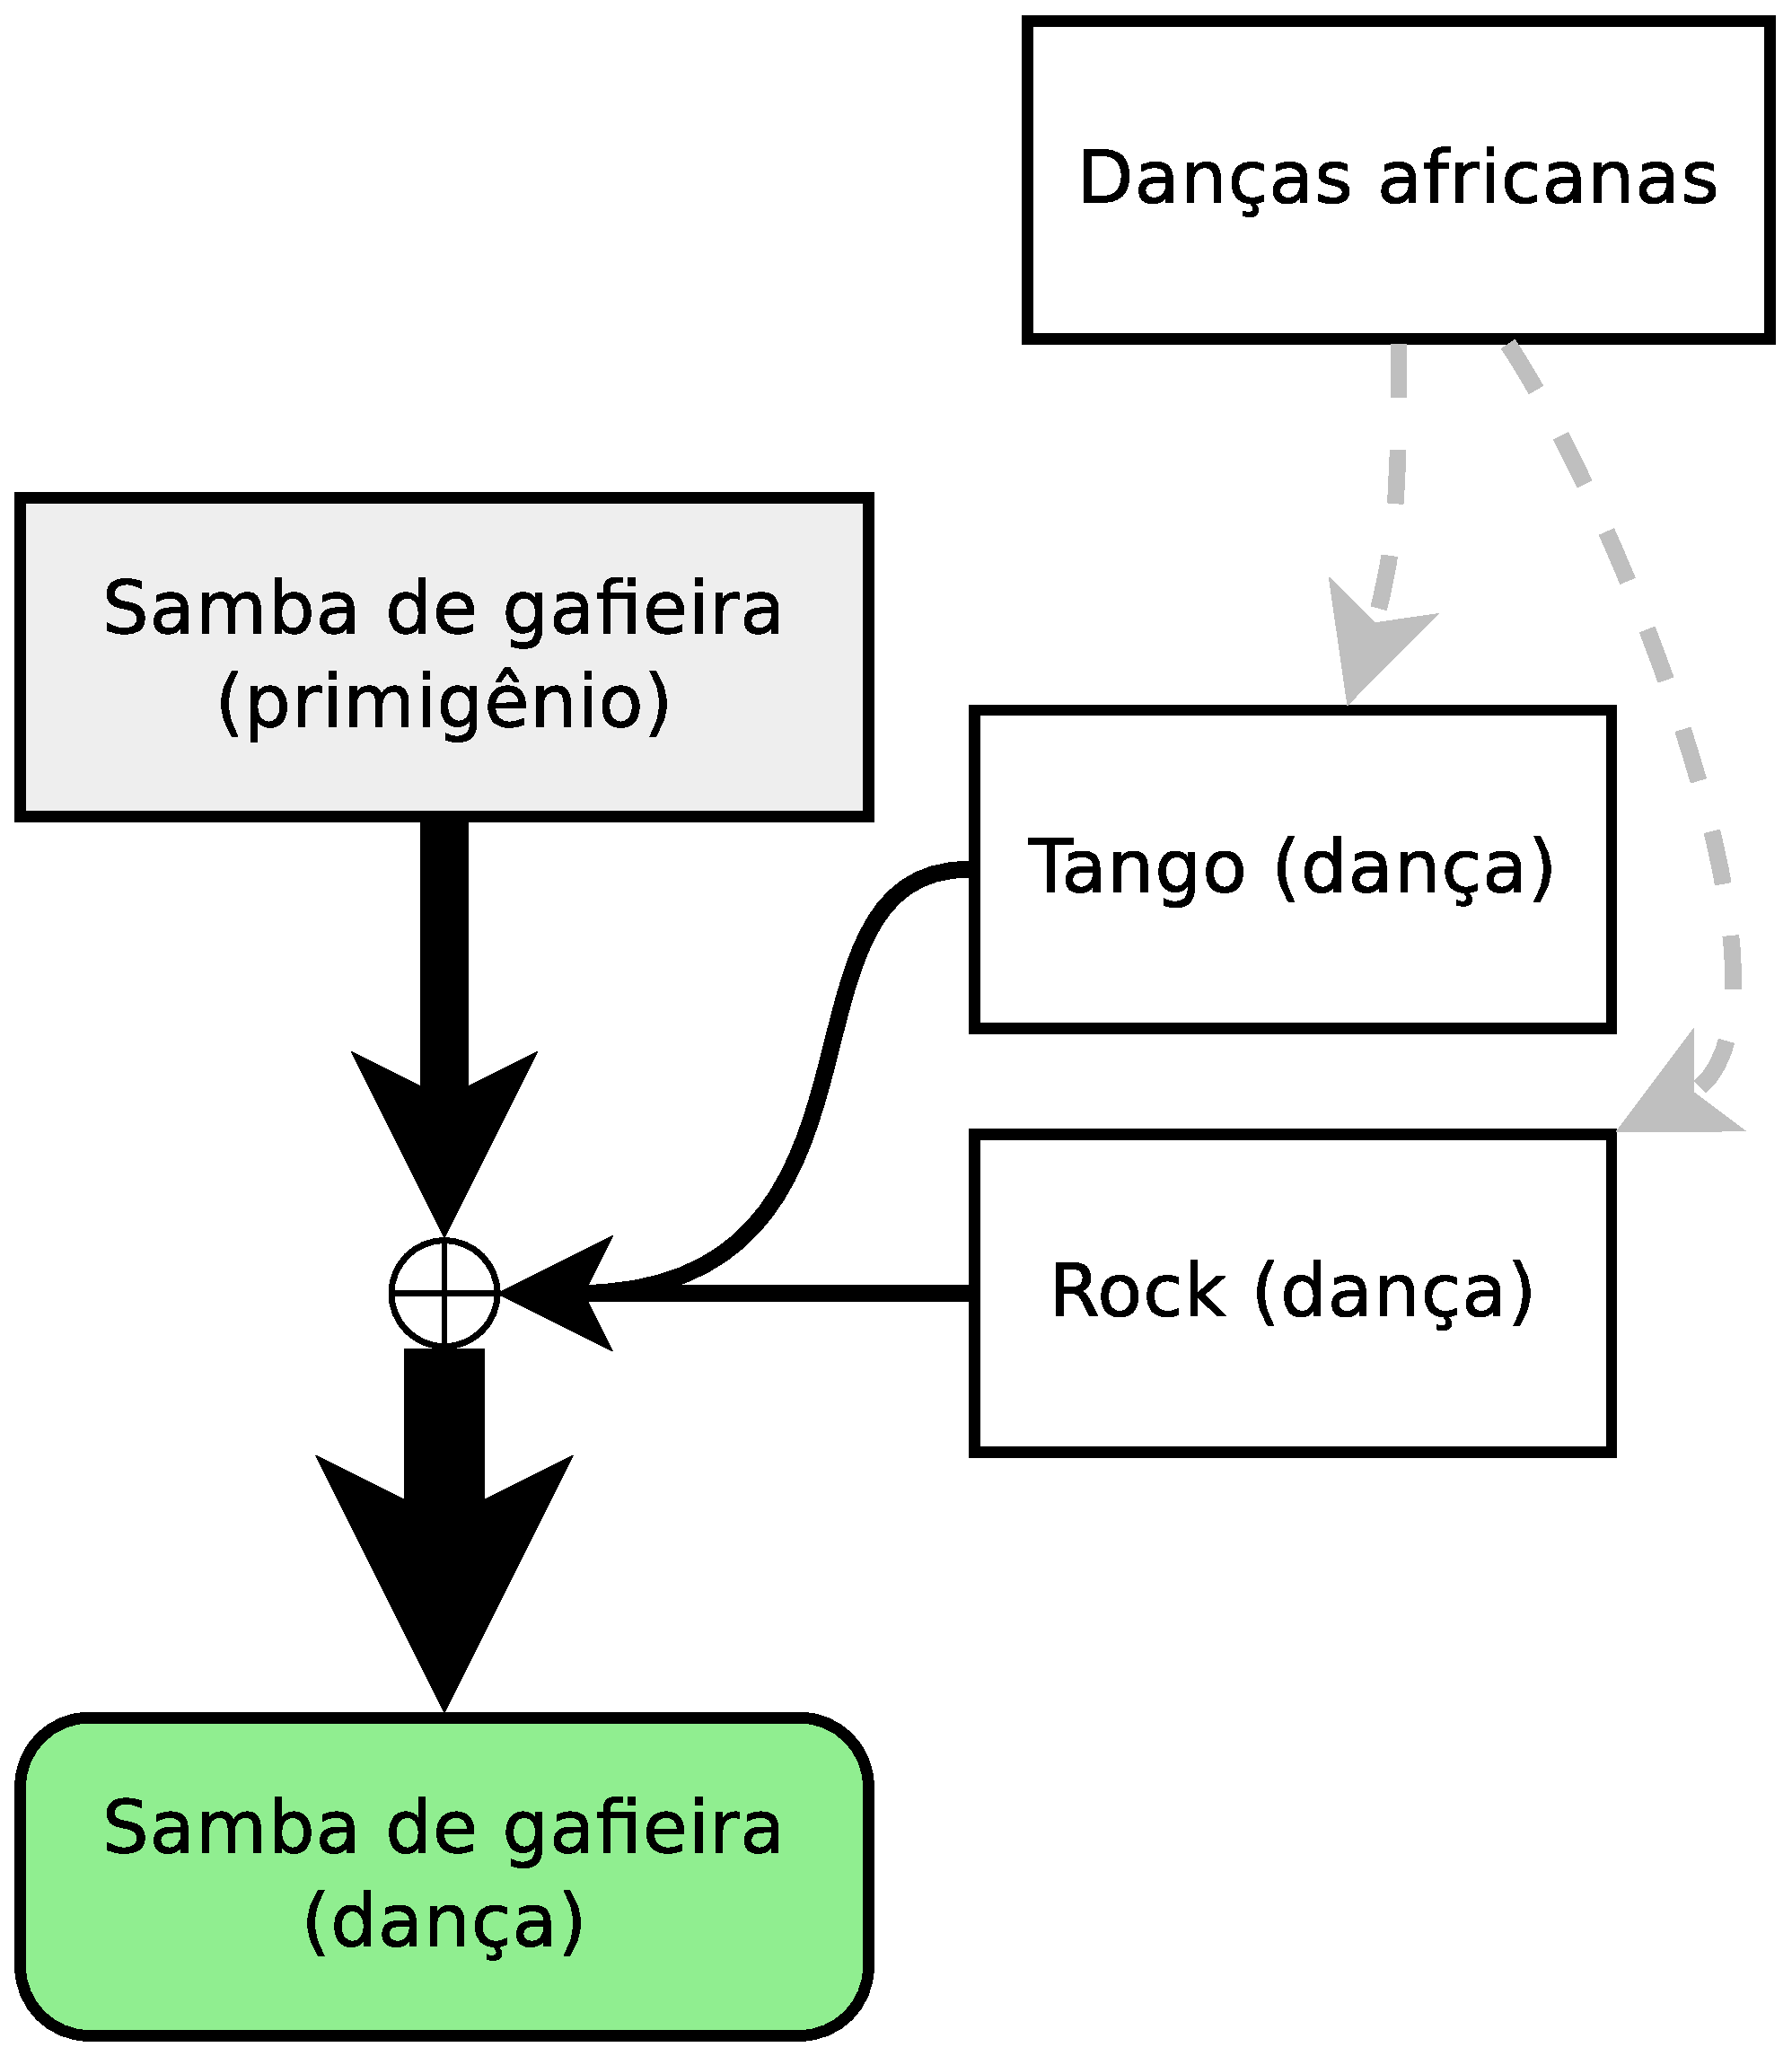
\includegraphics[width=\textwidth]{chapters/cap-historia-sambagafieira/sambagafieiraformula2.eps}
    \caption{Formação do samba de gafieira (atual).}
    \label{fig:formuladosambagafieira2}
  \end{subfigure}
\caption{Formula da criação do samba de gafieira.}
\label{fig:formuladosambagafieiraall}
\end{figure}


O aparecimento do samba nos salões de dança, 
foi um grande impacto para as pessoas que frequentavam estes lugares;
sendo considerado um ritmo novo e ligeiro,
que desagradou aos bailarinos de maior idade e menos ágeis \cite[pp. 6 - cad. B]{entrevistajuliojournalbrasil1}.
O senhor, Júlio Simões, Administrador da ``Kananga do Japão'' e posteriormente socio
do ``Elite Club'', chegou a temer pelo futuro do seus empreendimentos; porem, para sorte dele, 
o samba fez muito sucesso no Elite,
e passou a ser considerado vestibular indispensável para qualquer pessoa que pretendesse ser bailarino, 
compositor ou instrumentista \cite[pp. 6 - cad. B]{entrevistajuliojournalbrasil1}.

Pode-se estabelecer o ingresso do samba aos salões de dança numa época anterior e próxima da década de 1930,
dado que Júlio Simões, trabalhou na ``Kananga do Japão'' ate o ano de 1929 \cite[pp. 3 - cad. 3]{juliosimoes}  
\cite[pp. 11]{eliteinaugura} \cite[pp. 1 - cad. B]{gafieira2000reis}, pelo que sua preocupação sobre o samba 
nesse salão de dança deve ser anterior a essa data, porem não muito atrás dado que 
suas preocupações ainda eram vigentes na sua época no ``Elite Club'' 
que inciou em 1930 \cite[pp. 11]{eliteinaugura} \cite[pp. 3 - cad. 3]{juliosimoes} \cite[pp. 10]{simoesjournalbrasil1}.

\PRLsep{Os sambas nos salões em 1940}

O samba dançado nas gafieiras se firmou na década de 1940 \cite[pp. 142]{perna2002samba}. 
Em palavras do Prof. de dança Gino Fornaciari, 
a dança do samba praticada nos salões ou samba carioca (anterior a 1947 \cite[pp. 50]{fornaciari1947aprender}), 
 tinha um parecido com o Foxtrot e a Rumba, se dançava numa música sincopada com compasso binário,
sendo esta dança a preferida do mulato brasileiro
%sendo este estilo de dança de salão que nasceu na \hyperref[ref:batucadadanca]{\textbf{batucada}} 
%de pretos que descia à cidade na época das festas 
\cite[pp. 50-51]{fornaciari1947aprender}.


Na década de 1940 o samba dançado nos salões 
tinha 3 modalidades, samba-canção, samba-batucada e o samba liso \cite[pp. 58]{freitas1959danca} \cite[pp. 142-143]{perna2002samba} 
\cite[pp. 51]{fornaciari1947aprender}\cite[pp. 51]{fornaciari1950aprender}.\\
\begin{itemize}

\item \textbf{Samba-canção (dança):}
\index{Dança!Samba-canção} 

Este era uma dança com balanços aos lados que se executava de joelhos flexionados,
usando dois movimentos por cada compasso binario \cite[pp. 58]{freitas1959danca} 
\cite[pp. 51]{fornaciari1947aprender} \cite[pp. 143]{perna2002samba}; 
no ano 2001 se considera que este é um modo de dança extinto \cite[pp. 143]{perna2002samba}.

na Figura \ref{fig:samba-cancao-basico-frente} se mostra o passo básico para a frente do samba-canção,
e na  Figura \ref{fig:samba-cancao-basico-frente} o mesmo movimento para trás,
este eram usados antes de 1947 e inclusive no ano de 1959;
em ambos casos se usa os 2 movimentos antes mencionados, e a cor cinza indica a posição inicial \cite[pp. 51]{fornaciari1947aprender} \cite[pp. 59-60]{freitas1959danca}. 
\begin{figure}[h]
    \centering
    \begin{subfigure}[b]{0.4\textwidth}
        \centering
        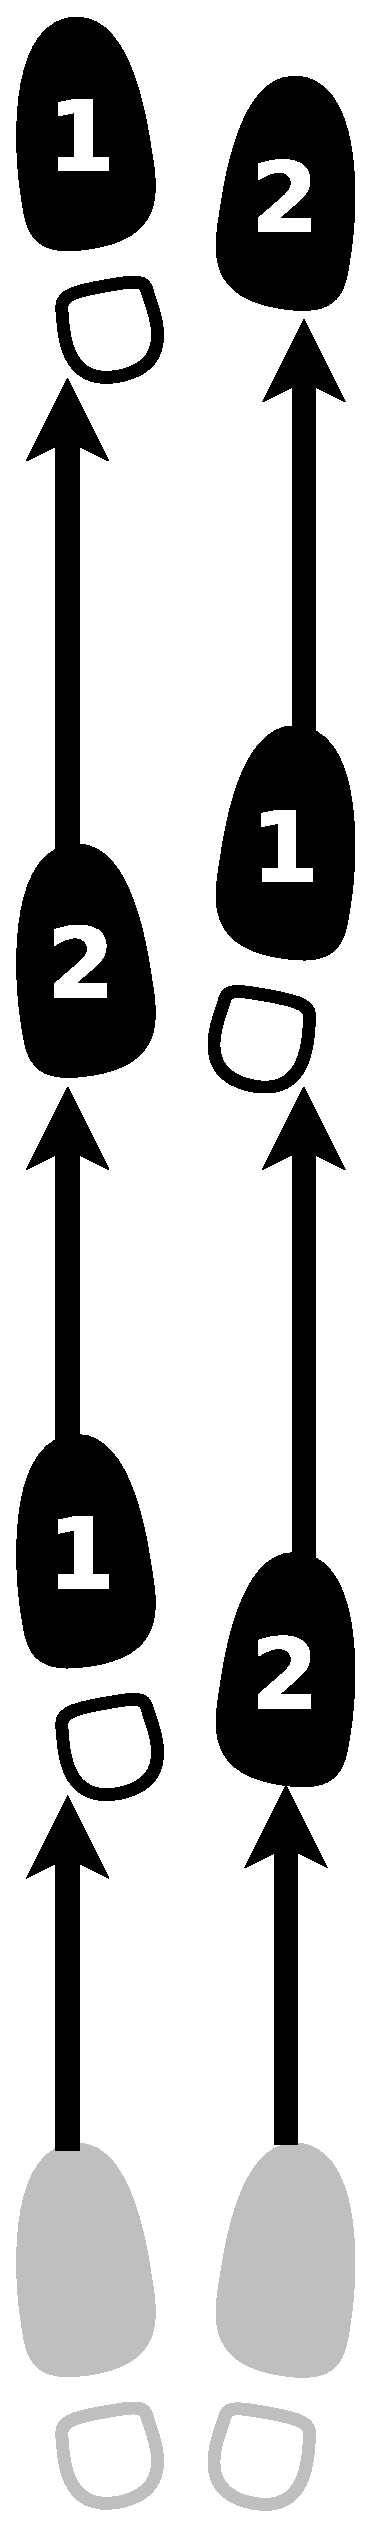
\includegraphics[width=0.25\textwidth]{chapters/cap-historia-sambagafieira/samba-cancao-basico-frente.eps}
        \caption{Passo básico para a frente.}
        \label{fig:samba-cancao-basico-frente}
    \end{subfigure}
    ~ %add desired spacing between images, e. g. ~, \quad, \qquad, \hfill etc. 
      %(or a blank line to force the subfigure onto a new line)
    \begin{subfigure}[b]{0.4\textwidth}
        \centering
	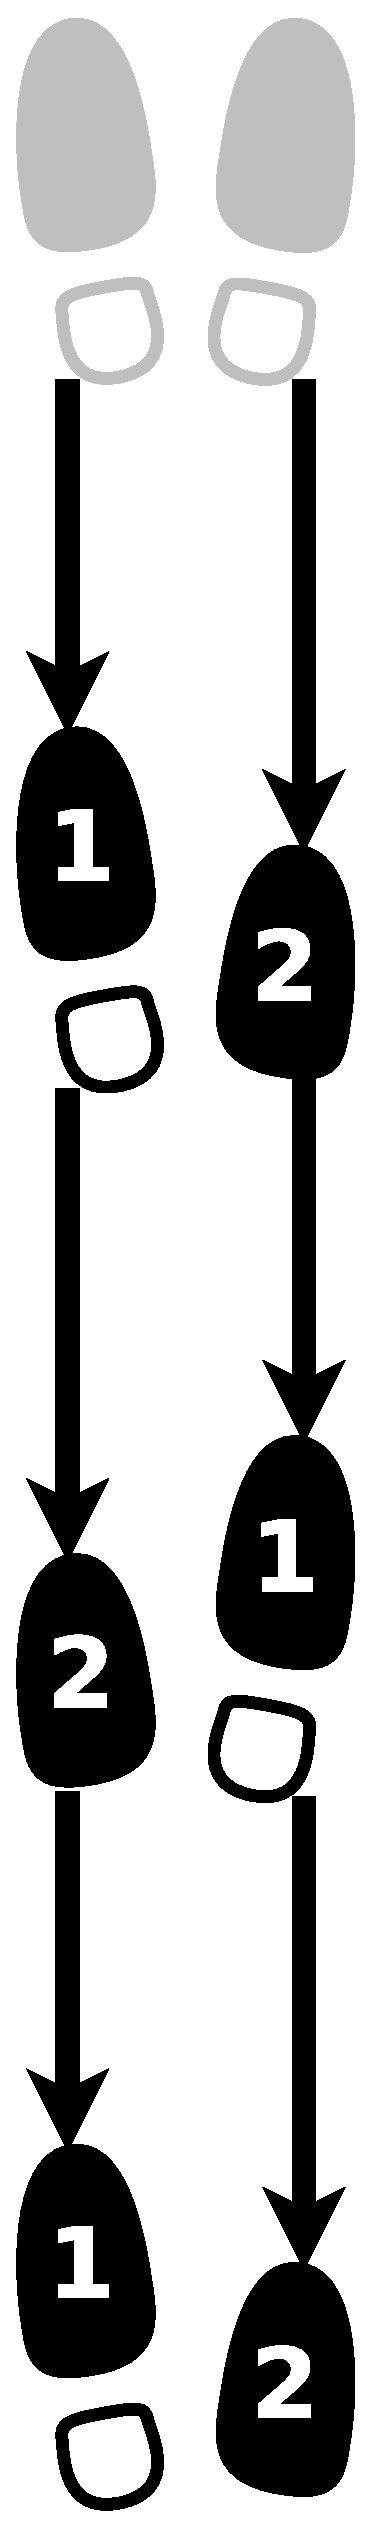
\includegraphics[width=0.25\textwidth]{chapters/cap-historia-sambagafieira/samba-cancao-basico-tras.eps}
        \caption{Passo básico para trás.}
        \label{fig:samba-cancao-basico-tras}
    \end{subfigure}
    \caption{Samba-canção da década de 1959.}\label{fig:samba-cancao-basico}
\end{figure}


\item \textbf{Samba-batucada:}
\index{Dança!Samba-batucada} 



Existe uma menção sobre este estilo no ``Jornal do Brasil'', no dia 9 de janeiro de 1938,
onde se indica \cite[pp. 4]{musicasambavariasdef1}:
\begin{citando}%%
Tentativas isoladas de puro 
snobismo e ás vezes de compreensão 
inexata da origem da 
musica e dansa, chamam-no de samba jongo, \textbf{samba batucada} ou
pretendem mistura-lo com o fox, -- samba fox ou com a rumba samba-rumba.
\end{citando}



No livro ``Feitiço decente: Transformações do samba no Rio de Janeiro (1917-1933)'' (2001),
se comenta, sobre uma roda do samba, que para o dançarino solista  escolher a seu sucessor podiam
existir duas modalidades, em ``samba liso'' (com umbigada) ou em ``samba duro'' 
(ou batucada) no qual a umbigada é substituída por uma pernada \cite[pp. 109]{sandroni2001feitico}.
Deste comentário pode ser deduzido de onde vem a denominação \textbf{samba-batucada}, 
que surgiu nos salões de dança apos 1930; pois já existia uma tradição na nomenclatura,
em separar duas formas de dançar uma mais leve (a liso) e uma mais brusca (batucada);
assim, a variante de samba no salão que tendia a explorar movimentos muito  gingados, bruscos ou rápidos,
foi nomeado de samba-batucada, em contraposição ao samba liso onde né se flexionavam os joelhos pra dançar.  



O samba-batucada era, desde antes de 1947 e inclusive ate 1959, uma dança com balanços que se dançava de joelhos flexionados  
e usava 3 movimentos por compasso, que exigia uma maior rapidez, 
especialmente no terceiro movimento que é mais rápido e curto \cite[pp. 61]{fornaciari1947aprender} \cite[pp. 58,66]{freitas1959danca};
seguindo essa descrição, 
o mais provável é que se dançara seguindo uma distribuição de tempos,
parecida ao ritmo do baião de 1949 \cite{CORTES2014}, como pode-se ver na Figura \ref{time:sambabatucada};
nela se exemplifica a distribuição de tempos em relação ao uso dos pés;
na segunda pisada de cada compasso só se usa a meia ponta do pé.
\begin{figure}[H]
\centering
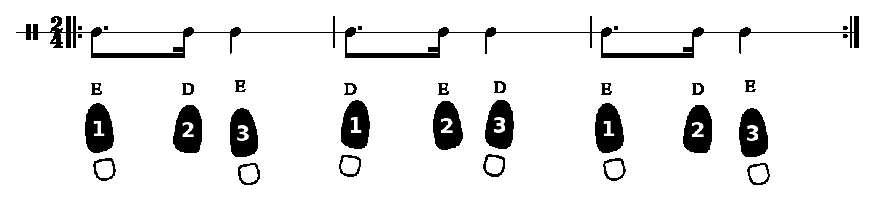
\includegraphics[width=\textwidth]{chapters/cap-historia-sambagafieira/sambabatucada.eps}
\caption{Ritmo das pisadas no samba-batucada.}
\label{time:sambabatucada}
\end{figure}

Sobre os passos de samba-batucada usados desde antes de 1947: 
A Figura \ref{fig:samba-batucada-basico-frente}  mostra o passo básico para a 
frente, do samba-batucada, 
%correspondente à distribuição de tempos da Figura \ref{time:sambabatucada},
e na  Figura \ref{fig:samba-batucada-basico-tras} temos o mesmo movimento para trás;
em ambos casos se usam passos em grupos de 3; a cor cinza indica a posição inicial \cite[pp. 61-62]{fornaciari1947aprender} \cite[pp. 63]{freitas1959danca}. 
\begin{figure}[h]
    \centering
    \begin{subfigure}[b]{0.4\textwidth}
        \centering
        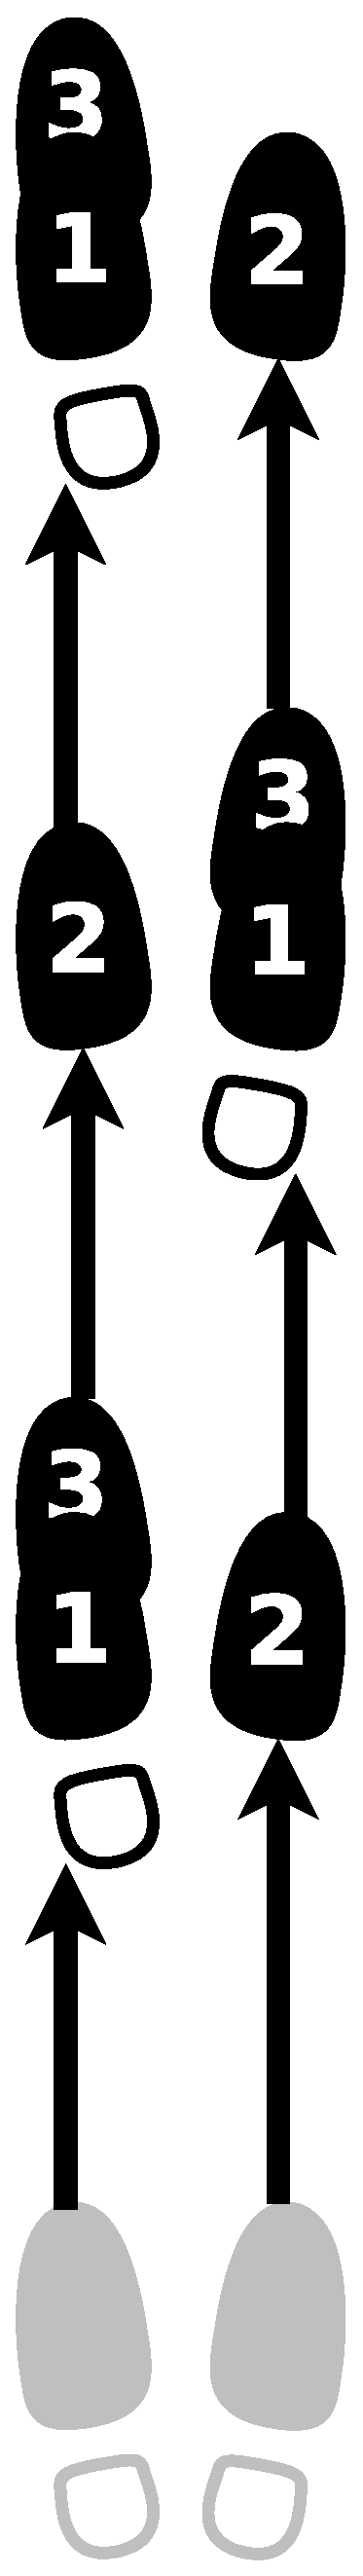
\includegraphics[width=0.25\textwidth]{chapters/cap-historia-sambagafieira/samba-batucada-basico-frente.eps}
        \caption{Passo básico para a frente.}
        \label{fig:samba-batucada-basico-frente}
    \end{subfigure}
    ~ %add desired spacing between images, e. g. ~, \quad, \qquad, \hfill etc. 
      %(or a blank line to force the subfigure onto a new line)
    \begin{subfigure}[b]{0.4\textwidth}
        \centering
	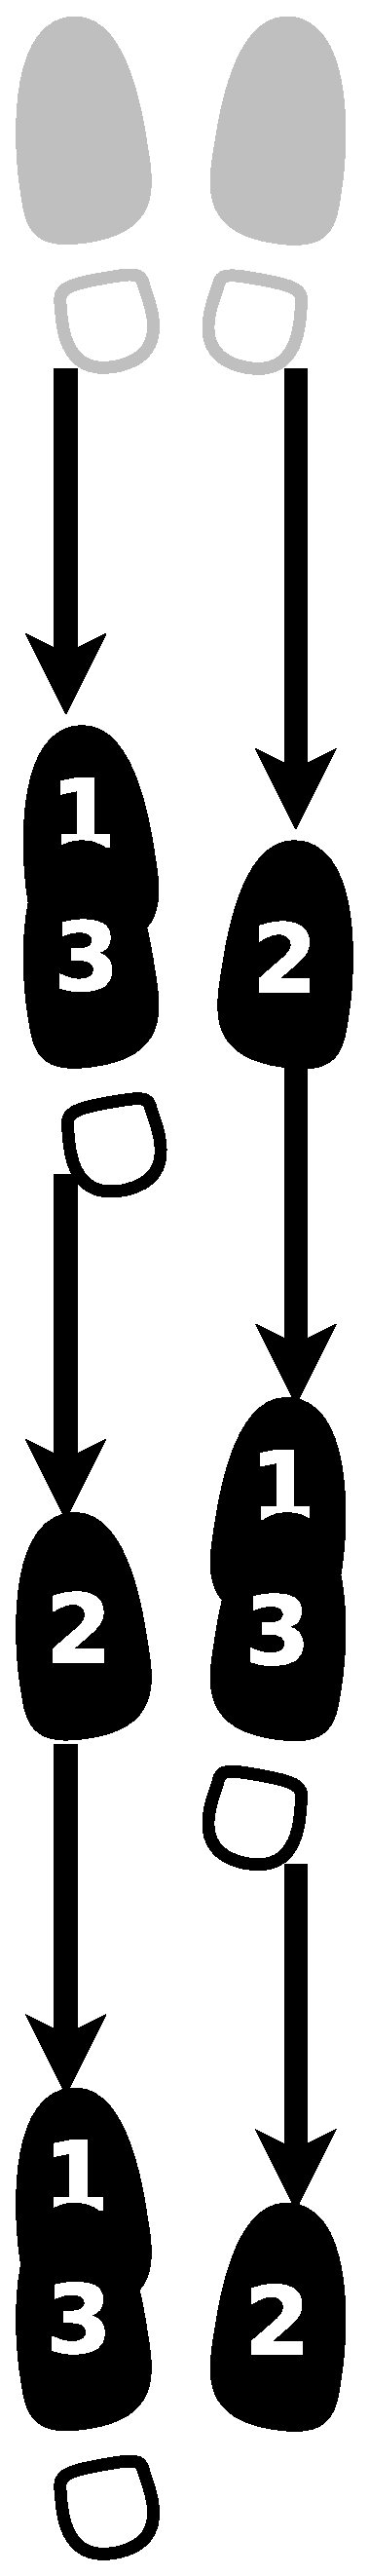
\includegraphics[width=0.25\textwidth]{chapters/cap-historia-sambagafieira/samba-batucada-basico-tras.eps}
        \caption{Passo básico para trás.}
        \label{fig:samba-batucada-basico-tras}
    \end{subfigure}
    \caption{Samba-batucada da década de 1959.}\label{fig:samba-batucada-basico}
\end{figure}

Outros passos conhecidos no ano de 1947, para este estilo de samba, tem nomes como: 
o pião, o balão, a cortada, a meia cortada, a joelhada, a patineta, e outros \cite[pp. 66]{fornaciari1947aprender}.
Para o Prof. Fornaciari, em São Paulo no ano de 1947 o pião e o balão são o mesmo movimento, 
sendo este o movimento mais importante do samba-batucada;
e a diferença do pião de \AnoLivro~ que se executa tradicionalmente em sentido horário,
o pião de 1947 se executava em sentido anti-horário \cite[pp. 68,72]{fornaciari1947aprender} 
\cite[pp. 73]{fornaciari1950aprender}.

Além dos estilos dançados nos salões, seguindo o Prof. Fornaciari, 
no ano de 1950 existem as danças estilizadas que estão orientadas 
para ser executadas em teatros \cite[pp. 149]{fornaciari1950aprender}. 
No caso do samba estilizado, este precisa de maior esforço físico dos dançarinos 
além de ser uma dança com maior flexibilidade, jogo de pernas, e com passos mais variados.
Por exemplo, no livro ``Como aprender a dançar'' (1950), temos um movimento que inicia com o condutor no abraço de dança,
e depois este dá uma patinada ou passo para atrás com a perna esquerda 
ao mesmo tempo que eleva ao seguidor \cite[pp. 160-1961]{fornaciari1950aprender};
este movimento  é muito similar a outro, chamado ``Elevador'', que é muito conhecido no samba de gafieira de \AnoLivro.
Nessa mesma página se explica outro movimento, esta vez chamado de ``cortada'', 
que não é outra coisa que uma pernada (presumivelmente só um contato leve) que o condutor da com sua perna esquerda,
sobre a perna direita do seguidor, um pouco abaixo do quadril\footnote{
Pessoalmente lembro ter visto este movimento ao contrario, quando um seguidor da esta pernada 
sobre a perna do condutor, um pouco abaixo do quadril, e o condutor aproveita para fazer uma sacada de perna,
inclusive tenho lembranças de telo visto no tango.}.
O livro também explica um movimento de samba estilizado chamado ``Joelhada'' \cite[pp. 160-1961]{fornaciari1950aprender}, 
que mas bem é uma postura, sendo esta muito similar à postura de ``Facão'' no samba de gafieira de \AnoLivro,
porem a postura do abraço é muito mais aberta, de modo que ao não estar colados,
o único ponto de contato entre os pares é a parte interna do joelho. 
Como uma semelhança mais com o facão,
no livro se indica que a joelhada pode ser executada apos o pião (do ano de 1947 que era em sentido anti-horário).
Outro movimento no samba estilizado é a ``calçada'', pela descrição feita no livro,
este movimento, é o que no samba de gafieira de \AnoLivro~ chamaríamos ou associaríamos com o ``Balão'' \cite[pp. 162]{fornaciari1950aprender},
com a diferença de que na versão explicada no livro, este movimento não termina numa ``cadeirinha'',
e simplesmente apos chegar ao lado da perna esquerda do condutor (que era quando acontecia a cadeirinha), 
o seguidor retorna ao lado direito do condutor. 

Finalmente o livro revela,
que o passo básico do samba estilizado é o passo básico do samba-batucada \cite[pp. 163]{fornaciari1950aprender},
assim, o termo samba estilizado indica uma versão melhorada do samba-batucada,
orientado para teatros e apresentações. Pela semelhança com os passos de samba de gafieira de \AnoLivro,
nos passos ``Elevador'', ``Balão'' e ``Facão'' podemos teorizar, de que a modalidade samba-batucada foi
a que finalmente se converteu ou aportou mais ao samba de gafieira atual.
Uma evidencia que sustenta esta ideia, a podemos encontrar no filme ``Aviso aos navegantes'' (1950) \cite[min. 40:35]{AtlantidaDance},
onde a partir do minuto 40:35 podemos ver uma apresentação de samba de salão (num teatro),
onde os dançarinos fazem os movimentos de elevador e balão, com uma sequencia de movimentos,
semelhante à descrita no livro ``Como aprender a dançar'' (1950) do Prof. Fornaciari.
Além de que em alguns momentos pode-se perceber movimentos de pés, 
com uma distribuição de tempos como na Figura \ref{time:sambabatucada},
dando maior força à hipótese de que essa era a distribuição de tempos para o samba-batucada nessa época. 
%O samba-batucada é o samba de gafieira (primigênio) \cite[pp. 143]{perna2002samba}.

\item \textbf{Samba liso:}
\index{Dança!Samba liso}

Era uma dança com balanços que se dançava sem flexionar os joelhos;
este é um estilo de dança que perdura ainda ate nossos 
dias \cite[pp. 58,62]{freitas1959danca} \cite[pp. 61]{fornaciari1950aprender} \cite[pp. 143]{perna2002samba}, 
para mais detalhes ver a Seção \ref{subsec:sambalisodef}.
\end{itemize}

\subsection{Evolução do samba nos salões}

Com o passar dos anos foram agregados elementos de outras danças a esse primitivo, samba de gafieira;
por exemplo, movimentos do tango e do rock \cite[pp. 142]{perna2002samba}, 
obtendo assim a forma de dança que vemos hoje em dia, ver Figura \ref{fig:formuladosambagafieira2}.

Asim, podemos falar do samba de gafieira como dança, só apos da aparição do samba nos
salões de dança abertos ao público, e a partir da criação do termo gafieira pra definir a estes lugares.
Com a mistura destes dois acontecimentos obtemos o termo, samba de gafieira,
que iniciou seu caminho na dança, mas como uma descrição do âmbito da dança (e da música), que como nome próprio.
Porem, a formação dos movimentos e corporalidade desta dança tem um caminho que data desde muito tempo atrás,
desde os batuques, dos morros e das rodas.


A primeira referencia achada\footnote{Que não quer dizer a primeira existente.} 
na ``Hemeroteca Digital Brasileira'' da Fundação Biblioteca Nacional,
foi na ``Revista da Semana''(RJ), no dia 25 de dezembro de 1948,
onde na seção ``Eros Volusia'', subseção ``O pitoresco da excursão'', se indica \cite[pp. 48]{sambagafieirarefbn}
\begin{citando}
Ensinando o samba aos ministros da República, 
fazendo o povo vibrar com o \textbf{samba de gafieira}, entusiasmando
o meio intelectual com seu francês muito doce,
contando coisas desconhecidas aos dançarinos francêses,
fazendo a dança brasileira figurar nos Archives Internationales de la Danse.
Eros Volusia satisfez o grande ideal de sua vida artística, sentindo-se contente
com o que realizou na França, embora a Europa não dê dinheiro a ninguém.
O lucro artístico é que compensa.
\end{citando}


A Figura \ref{fig:sambagafieiracrono} mostra a cronologia do uso do termo samba de gafieira. 

\begin{figure}[h]
  \centering
    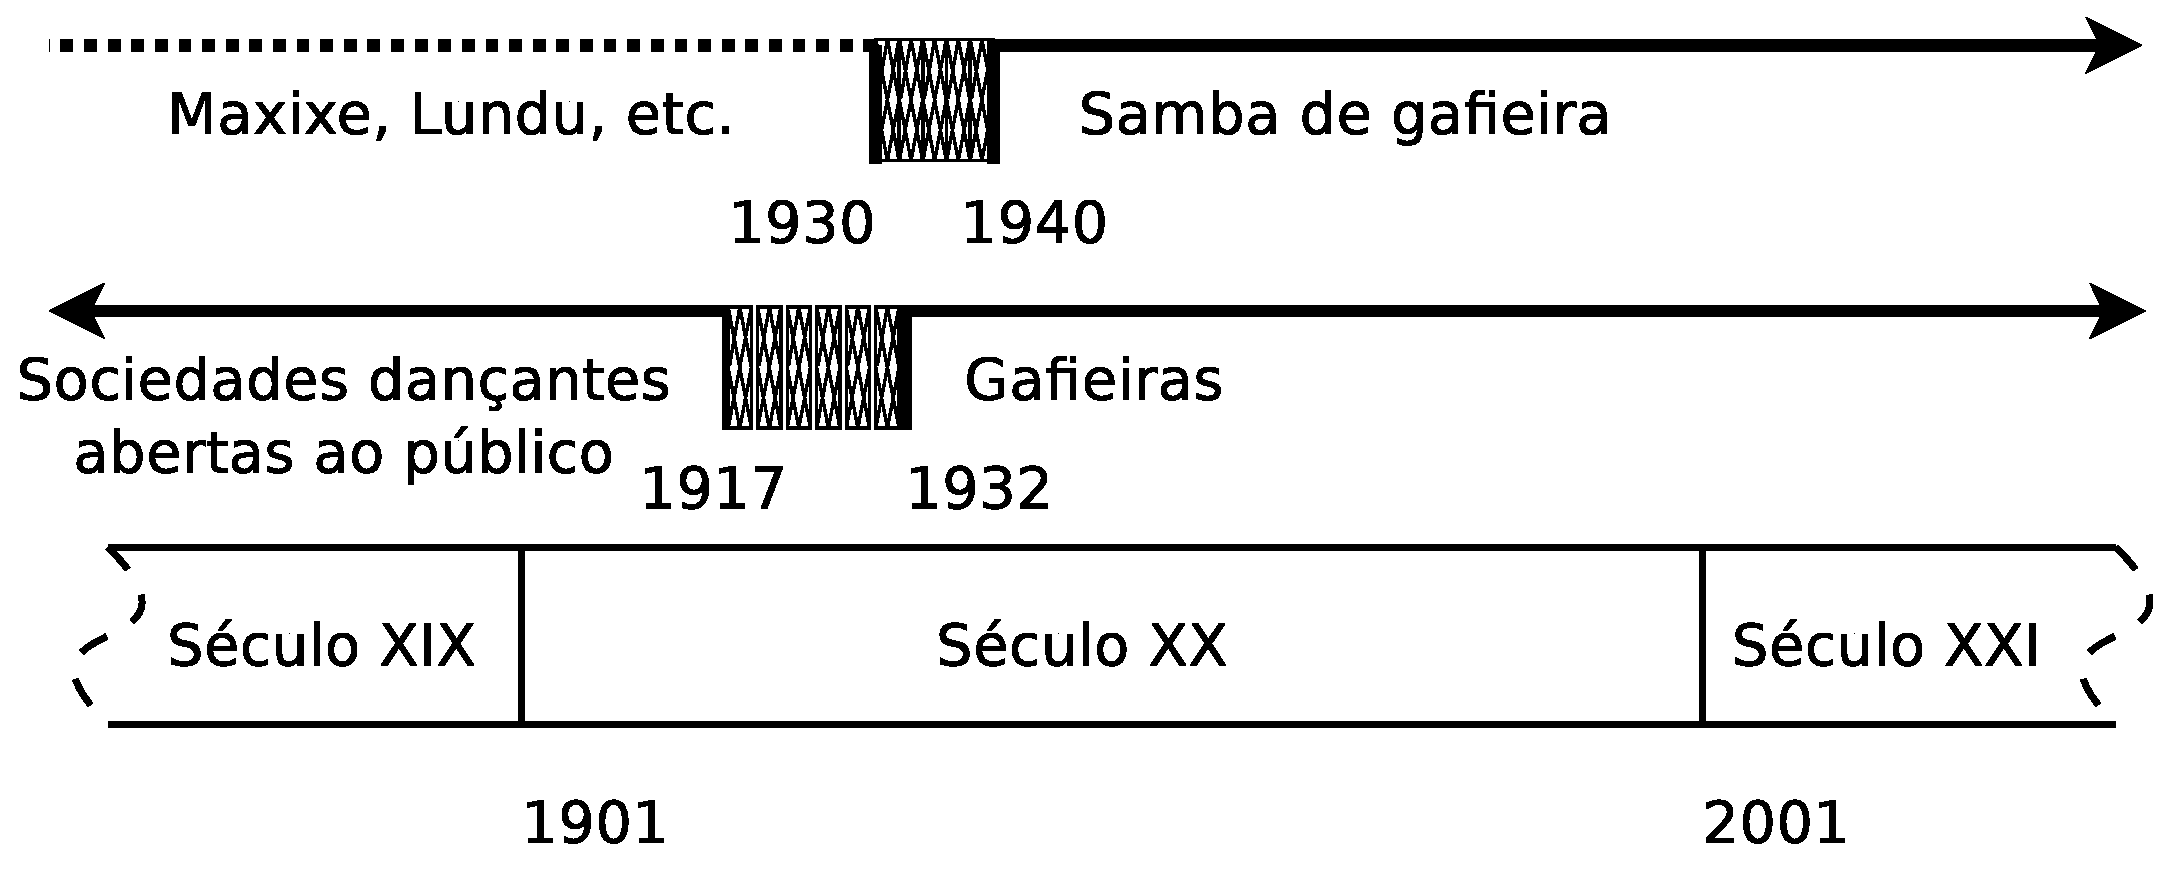
\includegraphics[width=1.0\textwidth]{chapters/cap-historia-sambagafieira/gafieira-crono.eps}
  \caption{ Cronologia da formação do samba de gafieira.}
\label{fig:sambagafieiracrono}
\end{figure}

%%%%%%%%%%%%%%%%%%%%%%%%%%%%%%%%%%%%%%%%%%%%%%%%%%%%%%%%%%%%%%%%%%%%%%%%%%%%%%%
%\clearpage
\section{Música para dançar samba de gafieira}
\label{subsec:gafieiradancaestilos}

Entre os estilos musicais em que o samba de gafieira (dança) se adapta bem, 
estão alguns dos subgêneros do samba; assim,
aqui mencionaremos algumas músicas que por sua graça, estilo e alegria,
a meu entender, podem ser dançados usando o samba de gafieira. Porem, 
estas músicas não pretendem ser máximos expoentes representativos do subgênero em que estão agrupados;
e sim uma indicação ou orientação ao leitor, 
para treinar sua dança usando músicas em que possa ser mais confortável a experiencia.

\begin{itemize}
\item \textbf{Samba de gafieira (música)}
\begin{example} ~
\begin{itemize}
%\item ``Samba de padua'' interpretado pelo grupo Turma da Gafieira.
\item ``Samba de morro'' interpretado pelo grupo Turma da Gafieira.
%\item ``Piston da gafieira'' de Billy Blanco, interpretado por Jorge Beiga.
\item ``Piston da gafieira'' de Billy Blanco, interpretado por Zeca pagodinho \cite{barbosa2014zeca}.
\item ``Beija-me'' de Roberto Martins e Mário Rossi, interpretado por Zeca pagodinho \cite{barbosa2014zeca}.
\item ``Pisei num despacho'' de Geraldo Pereira e Elpídio Viana, interpretado por Zeca pagodinho \cite{barbosa2014zeca}.
%\item ``Tive sim'' de Cartola, interpretado por Zeca pagodinho \cite{barbosa2014zeca}.
%\item ``Tarzan, o filho do alfaiate'' de Noel Rosa e Vadico, interpretado por Zeca pagodinho \cite{barbosa2014zeca}.
%\item ``Se você visse'' de Dino 7 cordas e Del Loro, interpretado por Zeca pagodinho \cite{barbosa2014zeca}.
\end{itemize}
\end{example} 

\item \textbf{Samba de breque}
\begin{example} ~
\begin{itemize}
\item ``Baile no elite'' interpretado por Casuarina.
\item ``Eu sou a marrom'' interpretado por Alicione.
%\item ``Hoje sou diferente'' interpretado por Lenita Rodrigues.
\item ``Pra levantar poeira'' interpretado por Bodhar.
\end{itemize}
\end{example} 

\item \textbf{Samba exaltação}
\begin{example} ~
\begin{itemize}
\item ``Aquarela do Brasil'' interpretado por Gal Costa.
\item ``Canta Brasil'' interpretado por Gal Costa.
\item ``Saudosa maloca'' interpretado pelo grupo Demônios da Garoa.
\end{itemize}
\end{example} 


\item \textbf{Pagode paulista (Sambalanço)}
\begin{example} ~
\begin{itemize}
\item ``Cheia de manias''  interpretado pelo grupo Raça Negra.
\end{itemize}
\end{example} 

\item \textbf{Partido alto}
\begin{example} ~
\begin{itemize}
%\item ``A língua'' interpretado por Beto lima.
\item ``Partido alto'' interpretado por Aleh.
\end{itemize}
\end{example} 

\item \textbf{Pagode}
\begin{example} ~
\begin{itemize}
\item ``Trilha do amor''  interpretado pelo Grupo Revelação. 
\item ``A batucada te pegou'' interpretado pelo Grupo Sou Muleke.
\item ``Dança da solidão'' interpretado por Pagode de Mesa do álbum Terra Brasil. 
\item ``Eu e você sempre'' interpretado por Jorge Aragão
\end{itemize}
\end{example} 

\item \textbf{Samba-canção (música)}
\begin{example} ~
\begin{itemize}
\item ``Só louco'' interpretado por Luiz Melodia.
\item ``Você é a fonte'' interpretado por  Quinteto em Branco e Preto.
\item ``Eu quero é sossego'' interpretado por Paulo Moura.
\end{itemize}
\end{example} 

\item \textbf{Bossa nova}
\begin{example} ~
\begin{itemize}
\item ``I don't know (Bossa mix)'' interpretado por Erika do álbum ``I don't know''
\item ``Human nature'' interpretado por Marcela Mangabeira.
\end{itemize}
\end{example} 


\item \textbf{Choro}
\begin{example} ~
\begin{itemize}
\item ``Choro de gafieira'' de Pixinguinha.
\item ``Chorinho de gafieira'' de Astor Silva.
\item ``Noites cariocas'' de Jacob do Bandolim.
\end{itemize}
\end{example} 


\item \textbf{Samba-choro}
\begin{example} ~
\begin{itemize}
\item ``Escurinho'' interpretado por Corina Magalhães.
\item ``Tico tico no fubá'' interpretado por Leci Brandão.
\end{itemize}
\end{example}

\end{itemize}

A Figura \ref{fig:gafieiradancaestilos} mostra um resumo de alguns dos 
subgêneros do samba onde pode ser dançado o samba de gafieira.
\begin{figure}[h]
  \centering
    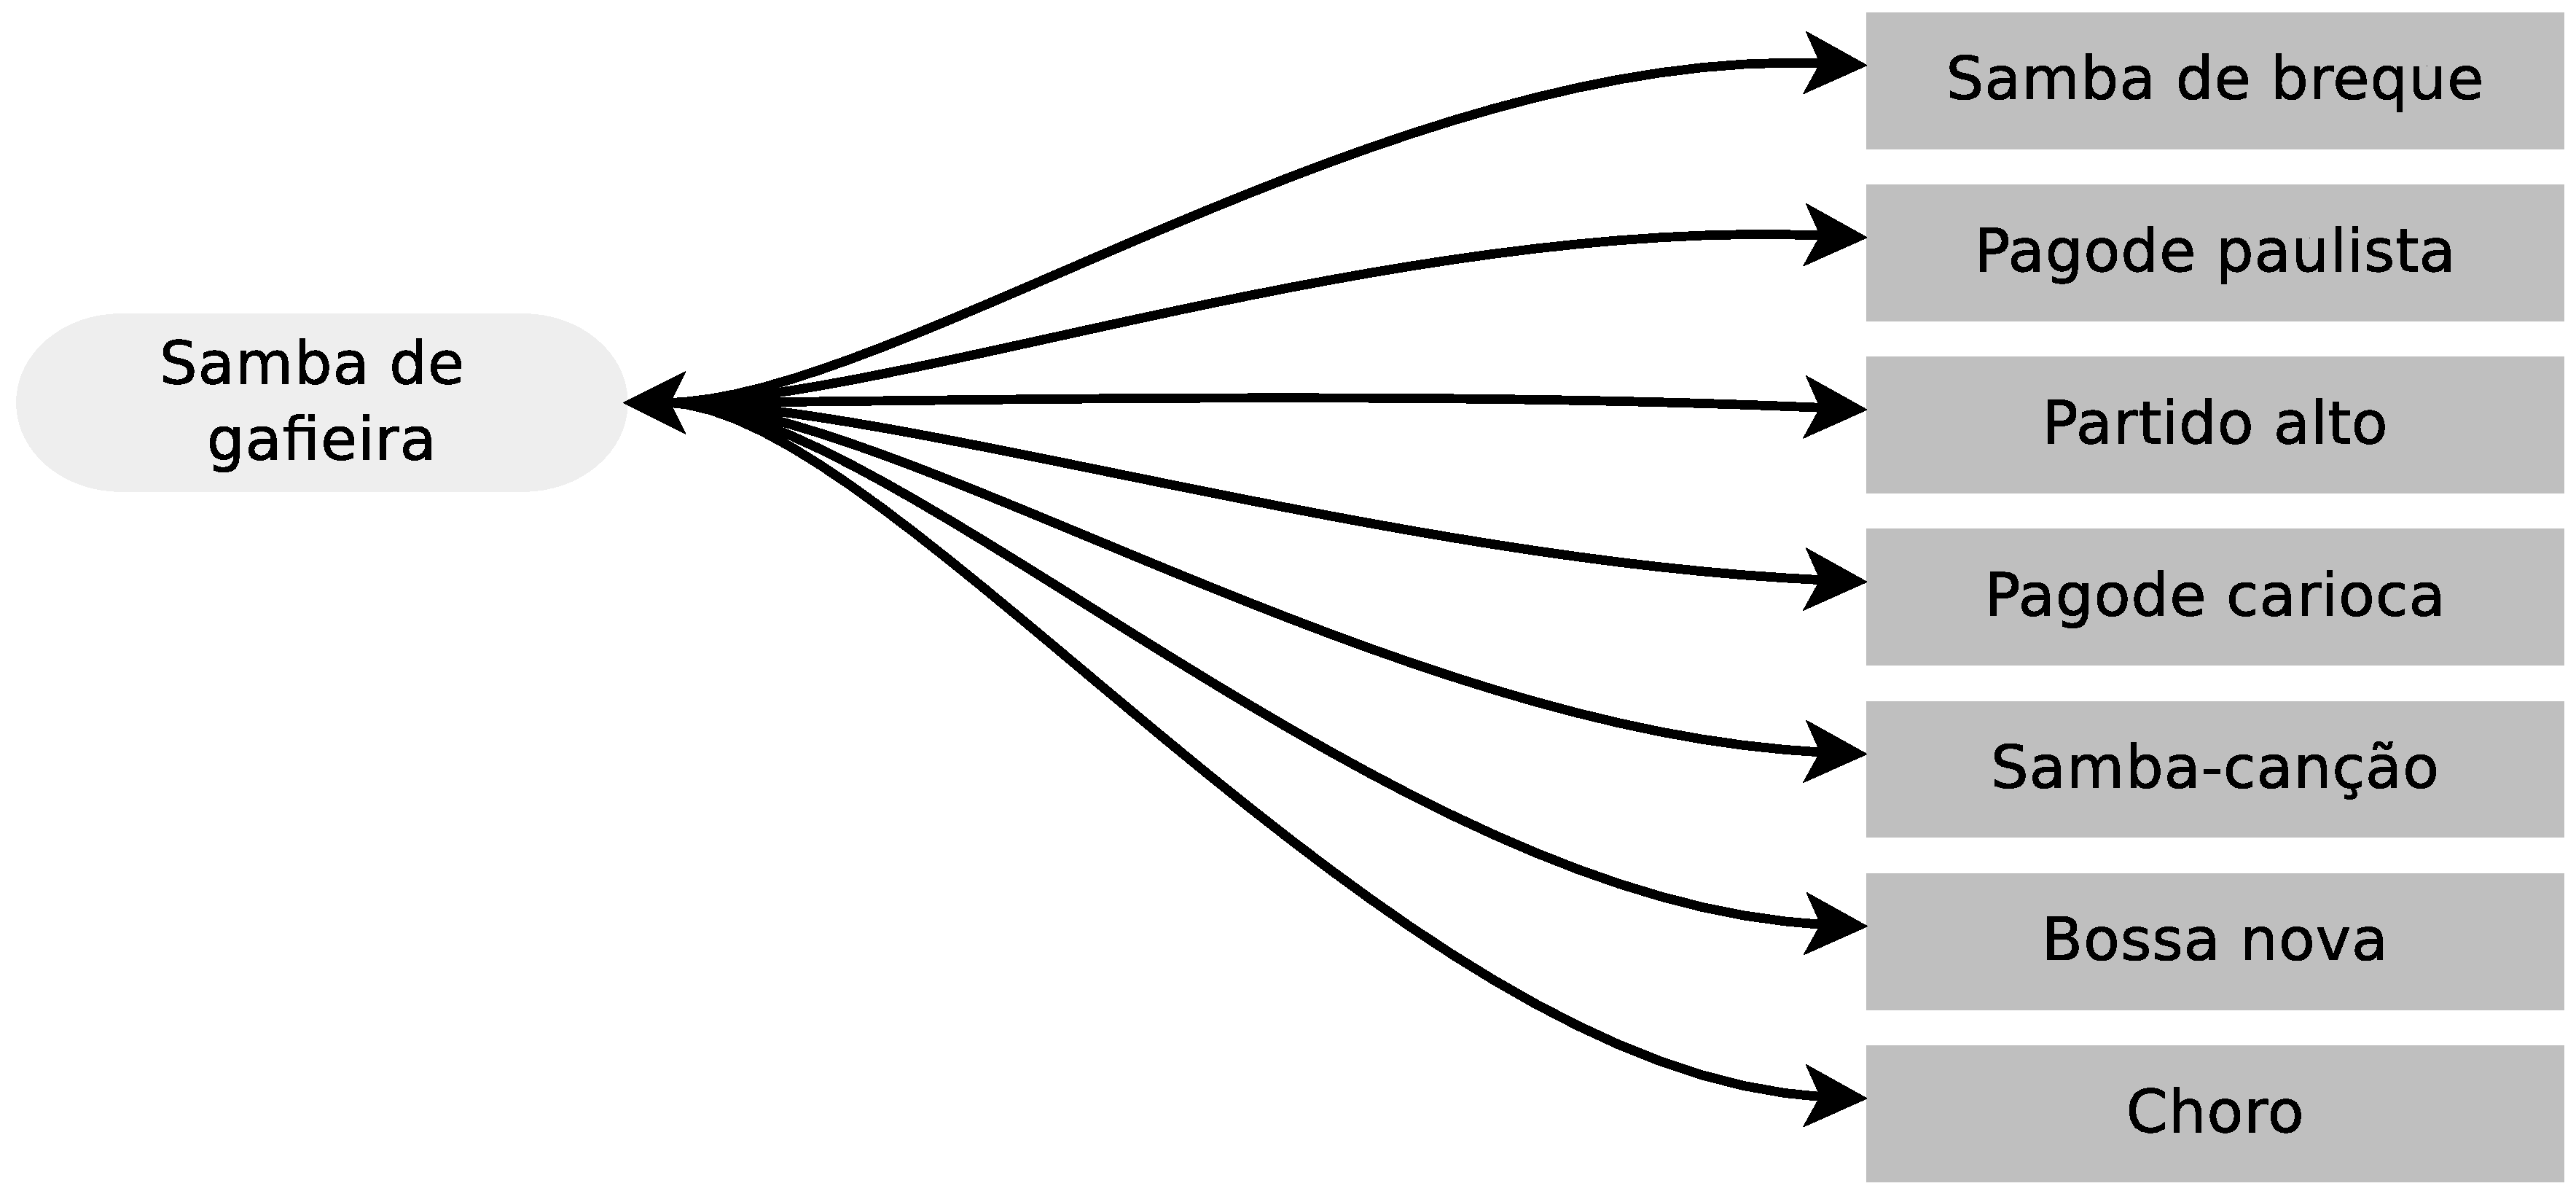
\includegraphics[width=0.9\textwidth]{chapters/cap-historia-sambagafieira/gafieiravcmusica.eps}
  \caption{ Subgêneros do samba onde pode-se dançar samba de gafieira.}
\label{fig:gafieiradancaestilos}
\end{figure}

